\chapter{\label{chap:modeling}Modelagem do Sistema}

Conforme visto na subseção \ref{subsec:simulation:components}, um sistema de
simulação possui uma série de componentes conceituais, cada um tendo suas
responsabilidades bem definidas. Para o projeto do simulador de sistemas de
elevadores deste estudo, doravante chamado apenas de simulador, optou-se pelo
paradigma de Programação Orientada à Objetos. Esta opção se deu pelos seguintes
motivos:

\begin{description}
  \item[Elevada Capacidade de Abstração]\hfill \\
    Conceitos da Programação Orientada à Objetos, como classes, interfaces,
    polimorfismo, herança e sobrecarga permitem a realização de uma modelagem
    conceitual em alto nível de abstração, permitindo uma explanação de fácil
    entendimento sem ser necessário abordar questões da implementação em si
    (linguagem de programação, arquitetura, etc).
  \item[Padrão de Mercado]\hfill \\
    Desde meados dos anos 90, a Programação Orientada à Objetos tornou-se o mais
    frequentemente utilizado no mercado de desenvolvimento de software e nos
    ambientes acadêmicos relacionados à computação. Assim, é possível atingir
    uma maior audiência.
  \item[Domínio dos Autores]\hfill \\
    O paradigma é de domínio dos autores deste estudo.
\end{description}

Nas próximas seções serão apresentadas as construções para o projeto do
simulador de elevadores.

\section{Eventos e Tipos}

A simulação de eventos discretos, como o próprio nome já diz, é totalmente
orientada à eventos. Isso significa dizer que as alterações no estado do sistema
ocorrerão somente na ocasião de algum evento. Sendo assim, é necessária uma
representação de um evento no projeto do simulador.

Um evento é uma estrutura que deve possuir as seguintes informações: (1) o tipo
do evento; (2) o horário agendado para a ocorrência do evento; (3) um cliente
(passageiro) e/ou (4) um elevador e/ou (5) um andar do prédio. As existência de
informações para os itens (3), (4) e (5) dependem do tipo de evento, que pode
ser uma das seguintes opções:

\begin{description}
  \item[Chegada de um cliente] \hfill \ um cliente chegou na fila de um andar
  \item[Chegada de um elevador] \hfill \ um elevador chegou a um andar e abriu as portas
  \item[Elevador moveu-se para cima] \hfill \ um elevador moveu-se para cima
  \item[Elevador moveu-se para baixo] \hfill \ um elevador moveu-se para baixo
\end{description}

Para o evento \textbf{chegada de um cliente}, é necessário conhecer o cliente e
o andar. Para o evento \textbf{chegada de um elevator}, é necessário conhecer o
elevador e o andar. Para os eventos \textbf{elevador moveu-se para cima} e
\textbf{elevador moveu-se para baixo}, é necessária a informação do elevador. A
figura \ref{fig:diagram:event} exibe o diagrama de classes para eventos e tipos
de evento.

\begin{figure}[htb!]
  \centering
  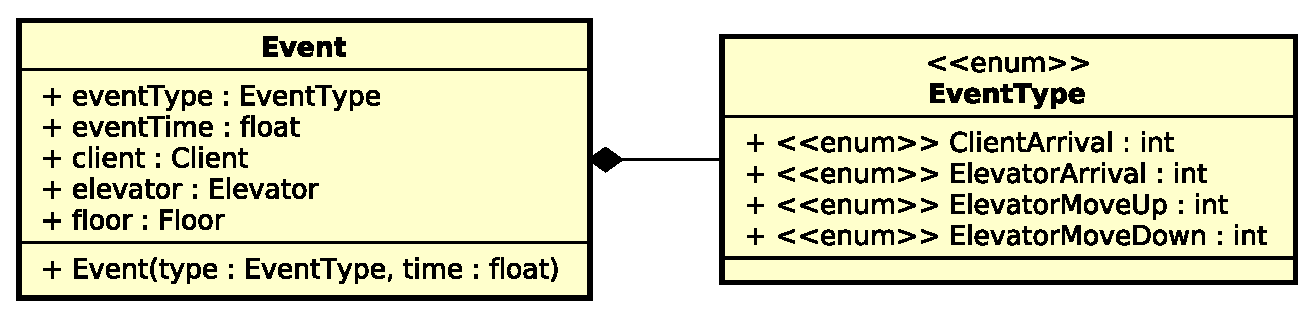
\includegraphics[scale=0.6]{img/event.eps}
  \caption{Classes para Eventos e Tipos de Eventos}
\label{fig:diagram:event}
\end{figure}

\section{Classes Singleton}

\textbf{Essa seção tá bem ruim. Melhorar bastante (ou até mesmo removê-la).}

Durante a modelagem desde projeto, fez-se o uso do pattern Singleton em algumas
entidades concretas. Uma classe Singleton significa que só é possível instanciar
um objeto daquela classe, sendo esta instância acessível à partir de qualquer
classe sem a necessidade de passagem de parâmetros.

Tecnicamente é coisa de preguiçoso, mas simplifica algumas coisas.

\section{Notificando Eventos: o pattern Observer}

Em um simulador, há a necessidade de executar diferentes ações na ocasião de um
evento específico. Por exemplo, atualizar o estado atual do sistema, as
estatísticas e o relógio da simulação. De acordo com Gamma
\cite{Gamma:1995:DPE:186897}, um \textit{design pattern} da programação
Orientada à Objetos indicado para o problema de notificar componentes que um
determinado evento ocorrereu é chamado de \textit{Observer}. Este
\textit{pattern} define uma dependência de um-para-muitos entre objetos de modo
que, quando este um objeto tem seu estado alterado, todos os seus dependentes
são notificados automaticamente. Por consequencia, estes objetos podem modificar
seu estado interno baseando-se nas informações desta notificação.

A figura \ref{fig:diagram:notification} ilustra as classes projetadas deste
sistema de Notificação de Eventos. A interface \textit{EventObserver} deve ser
realizada por qualquer classe que deseje receber eventos. Já a interface
\textit{EventNotifier} define a interface pública de um notificador de eventos.
Esta interface provê métodos que objetos \textit{EventObserver} possam se
registrar ou desregistrar para receber notificações das ocorrências de um
determinado tipo de evento, além de um método para realizar a notificação
propriamente dita do evento.

\begin{figure}[htb!]
  \centering
  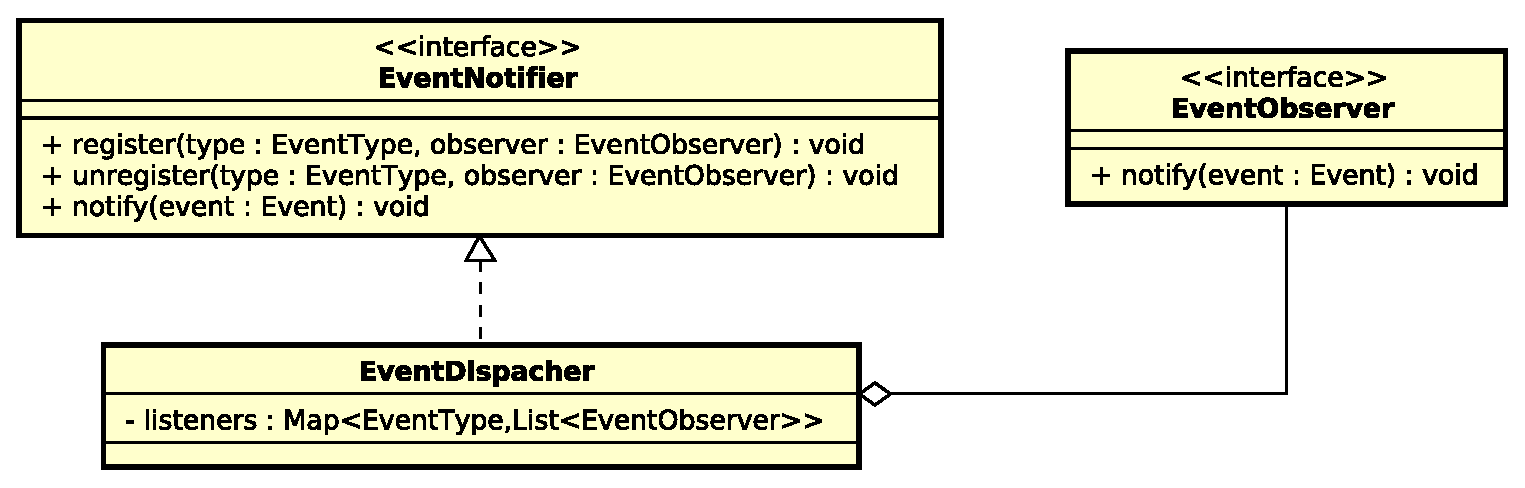
\includegraphics[scale=0.6]{img/notification.eps}
  \caption{Diagrama de Classes do Notificador de Eventos}
\label{fig:diagram:notification}
\end{figure}

A classe concreta \textit{EventDispatcher} realiza a interface
\textit{EventNotifier}. Para armazenar os objetos que deverão receber
notificações para cada evento, é utilizado um mapa que relaciona tipo de evento
com uma lista de \textit{EventObservers}. Na ocasião da ocorrência de um evento,
o \textit{EventDispatcher} é responsável por varrer a sua lista interna de
assinantes e notificá-los conforme o tipo de evento ocorrido.

Esta construção é bastante útil no momento em que possuímos três importantes
componentes do sistema que necessitam alterar o seu estado interno a cada evento
ocorrido (figura \ref{fig:diagram:observers}). São eles: \textit{Timer},
responsável por encapsular o relógio da simulação; \textit{Statistics},
responsável pela acumulação das estatísticas da simulação; e \textit{Building},
entidade que armazena o estado do prédio em si, com seus andares, elevadores e
passageiros. Na ocorrência de um evento, estas três entidades devem ser
notificadas e cada uma irá alterar seu estado interno da forma que lhe convir.

\begin{figure}[htb!]
  \centering
  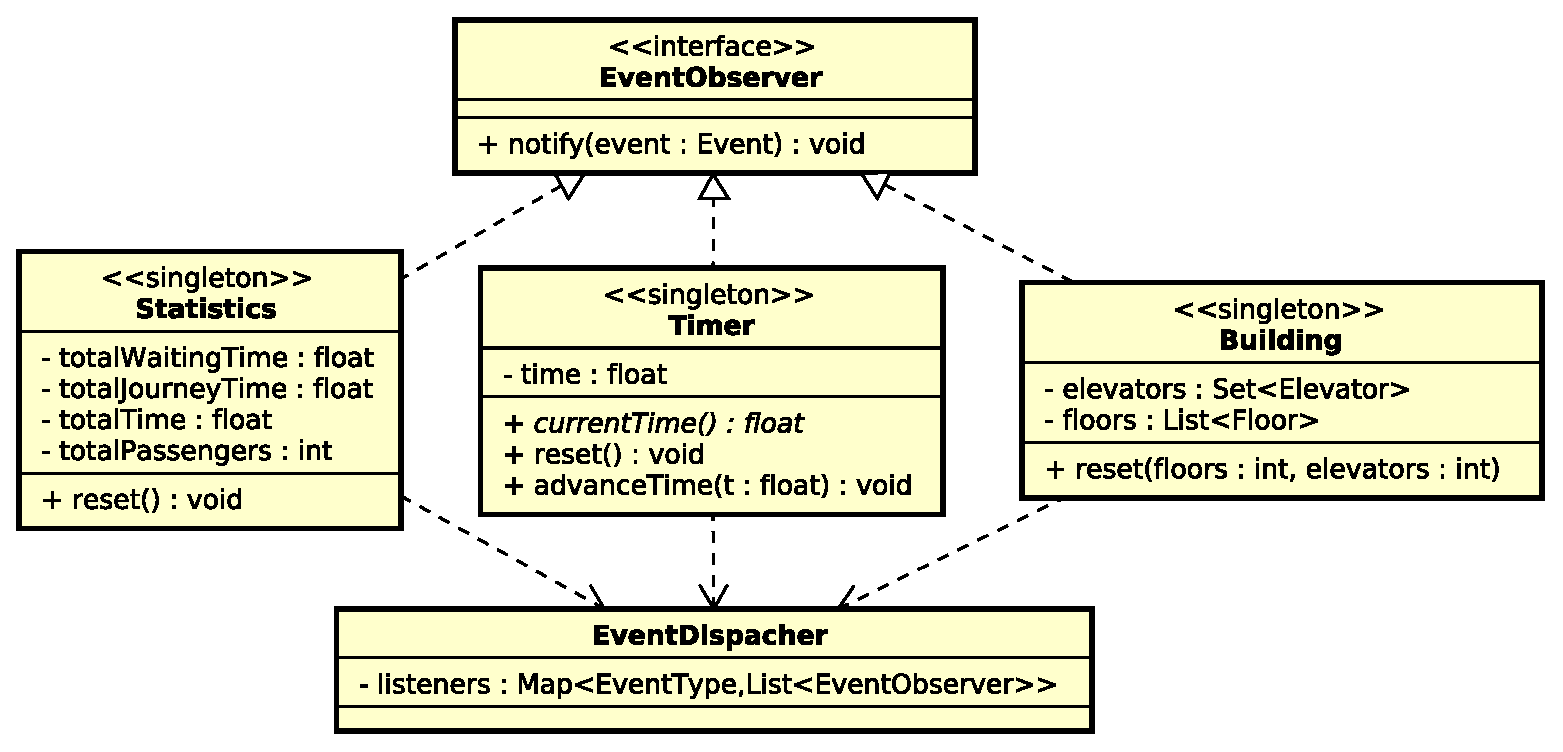
\includegraphics[scale=0.6]{img/observers.eps}
  \caption{Diagrama de Classes dos Observadores de Eventos}
\label{fig:diagram:observers}
\end{figure}

\section{Criação e Gerenciamento de Eventos}

\begin{figure}[htb!]
  \centering
  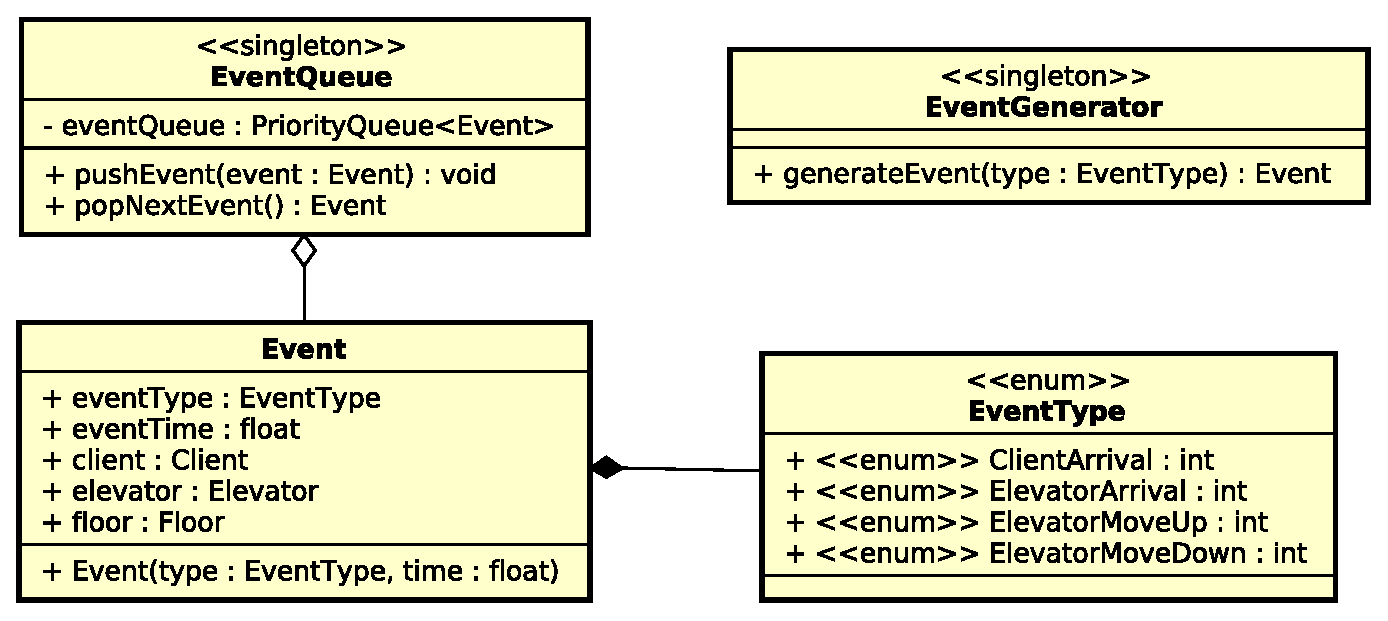
\includegraphics[scale=0.6]{img/event_management.eps}
  \caption{Diagrama de Classes do Gerenciador de Eventos}
\label{fig:diagram:event:manage}
\end{figure}

A criação de eventos ocorre na classe \textit{EventGenerator}.

A classe EventQueue gerencia a fila de eventos. Atraveś de uma PriorityQueue
(fila de prioridades), é possível armazenar eventos e ordená-los
automagicamente. A prioridade é inversamente proporcional ao tempo de ocorrência
de cada evento - ou seja, eventos mais próximos na linha do tempo terão uma
prioridade maior e ficarão primeiro na fila.

\begin{figure}[htb!]
  \centering
  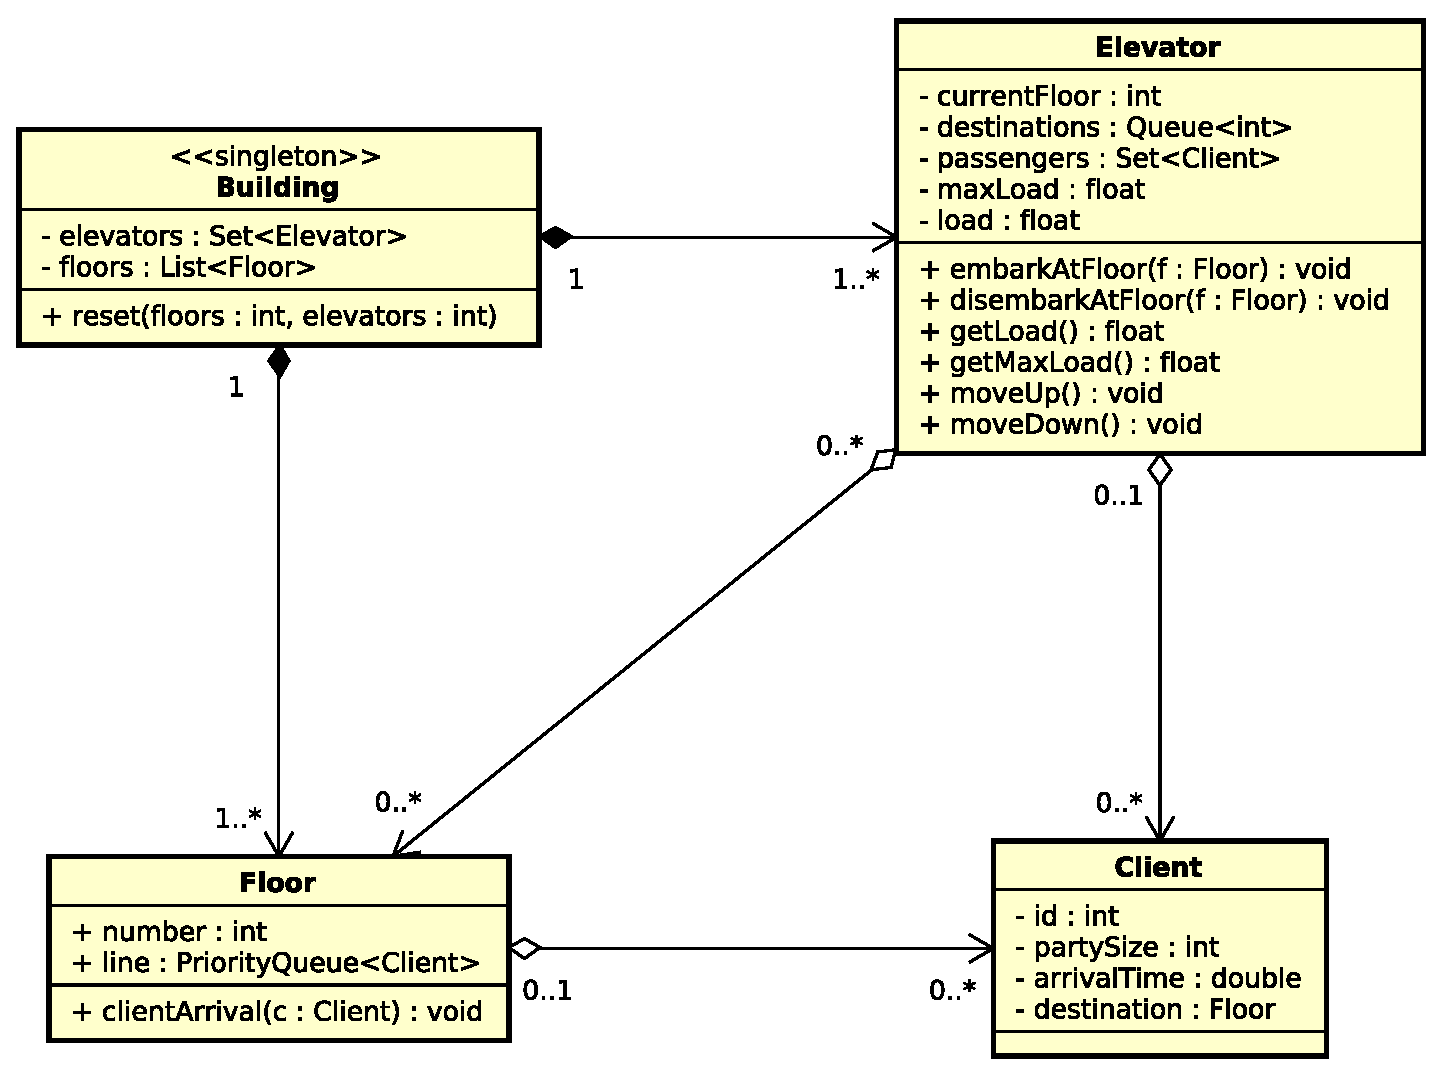
\includegraphics[scale=0.6]{img/state.eps}
  \caption{Diagrama de Classes da Representação do Estado do Sistema}
\label{fig:diagram:system}
\end{figure}

Por fim, a figura \ref{fig:diagram:simulator} ilustra o diagrama do simulador
com todas as classes (com exceção das classes Elevator, Client e Floor). Algumas
relações de menor relevância foram omitidas para uma melhor legibilidade.

\begin{figure}[htb!]
  \centering
  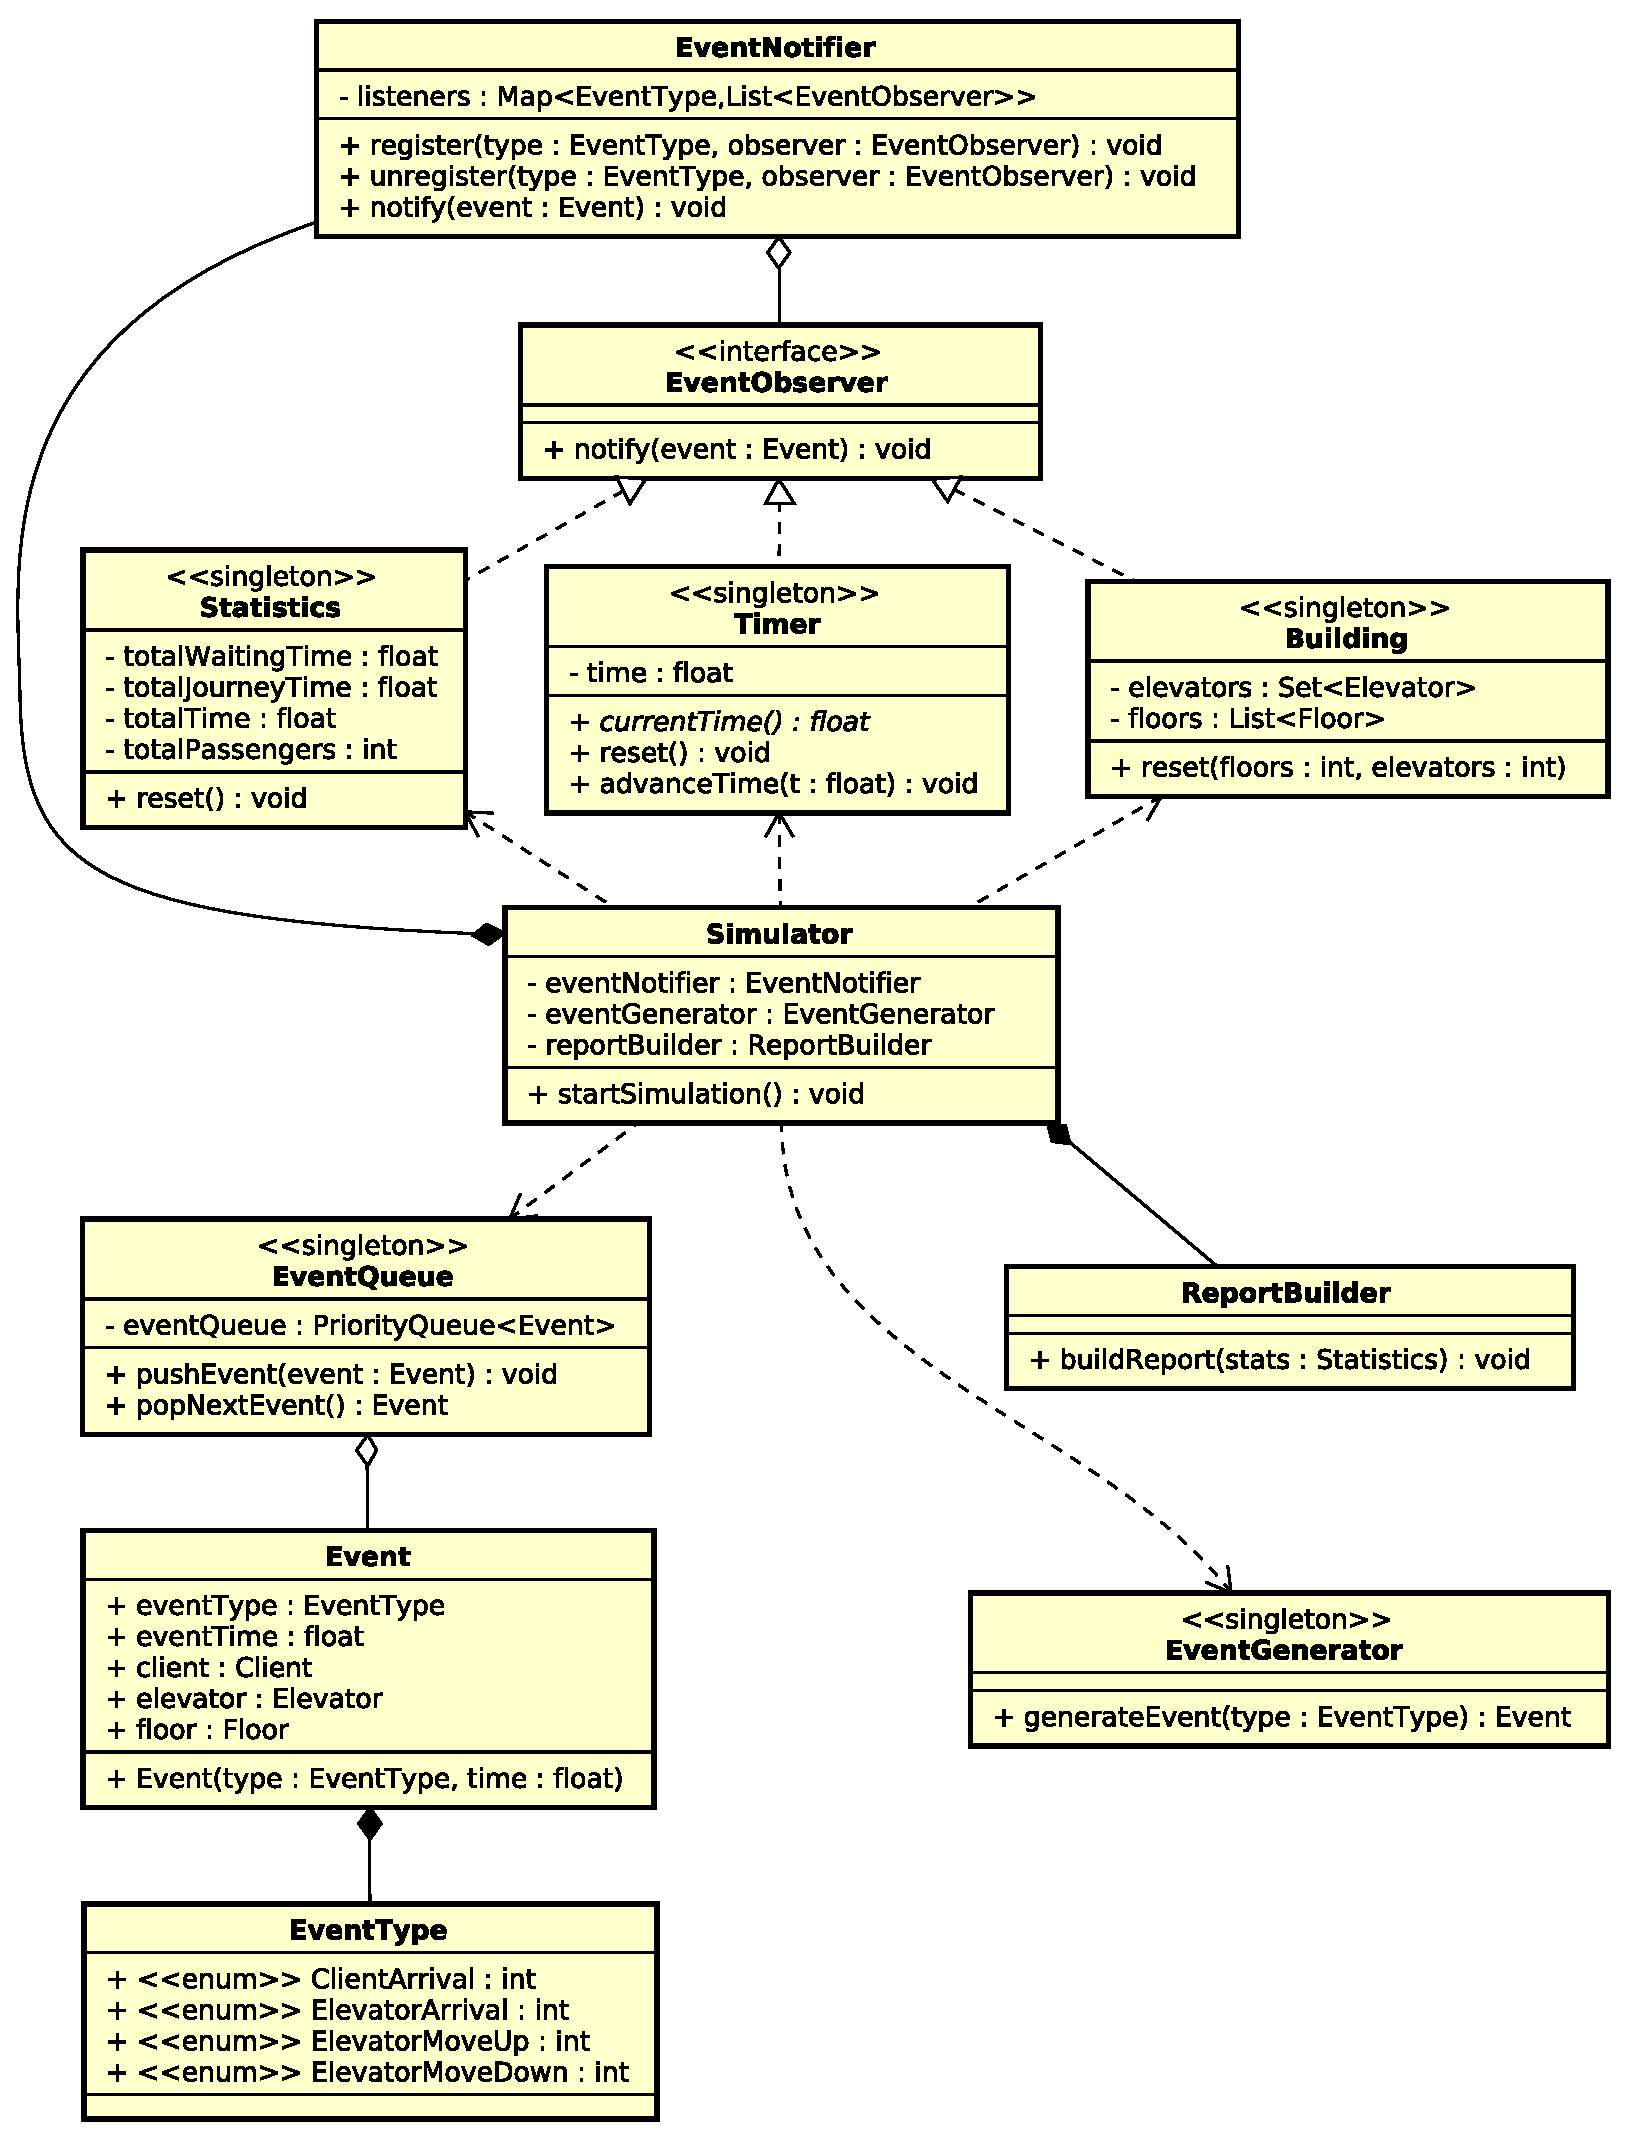
\includegraphics[scale=0.6]{img/simulator.eps}
  \caption{Diagrama de Classes do Simulador}
\label{fig:diagram:simulator}
\end{figure}


\subsection{aaaaaaaa}

Aqui vamos apresentar:

\begin{itemize}
  \item Descrições e diagramas UML dos componentes (classes, algoritmos, etc)
que dão sentido à simulação - ou seja, o modelo do sistema de elevadores
  \item Algoritmos e fluxogramas dos eventos do simulador que causarão
alterações no estado do sistema quais informações desejamos que o simulador
calcule para nós.
\end{itemize}

\section{\label{chap:input}Entrada de Distribuição de Probabilidade}

Aqui vamos apresentar:

\begin{itemize}
\item Conceitos sobre distribuições de probabilidade;
\item Conceitos sobre geração de variáveis aleatórias em ambiente computacional;
\item Descrever o modelo selecionado de processo de chegada de clientes
(passageiros);
\item Algoritmos e fluxogramas dos eventos do simulador que causarão alterações
no estado do sistema.
\end{itemize}